\documentclass[11pt,letterpaper]{article}

\newenvironment{proof}{\noindent{\bf Proof:}}{\qed\bigskip}

\newtheorem{theorem}{Theorem}
\newtheorem{corollary}{Corollary}
\newtheorem{lemma}{Lemma} 
\newtheorem{claim}{Claim}
\newtheorem{fact}{Fact}
\newtheorem{definition}{Definition}
\newtheorem{assumption}{Assumption}
\newtheorem{observation}{Observation}
\newtheorem{example}{Example}
\newcommand{\qed}{\rule{7pt}{7pt}}

\newcommand{\solution}[4]{
\thispagestyle{plain} 
\newpage
\setcounter{page}{1}
\noindent
\begin{center}
\framebox{ \vbox{
\vspace{4mm}
\vspace{0.2in} 
{\centering \large\mbox{#3}}\\
\vspace{0.1in}
{#1 \hfill {Date: #2}}
}}
\end{center}
\markright{#1}
}

\newenvironment{algorithm}
{\begin{center}
\begin{tabular}{|l|}
\hline
\begin{minipage}{1in}
\begin{tabbing}
\quad\=\qquad\=\qquad\=\qquad\=\qquad\=\qquad\=\qquad\=\kill}
{\end{tabbing}
\end{minipage} \\
\hline
\end{tabular}
\end{center}}

\def\Comment#1{\textsf{\textsl{$\langle\!\langle$#1\/$\rangle\!\rangle$}}}



\usepackage{graphicx, amssymb, amsmath, listings, float, mathtools}
\usepackage{color, url}
\usepackage{romannum}
\lstset{language = Python}
\lstset{breaklines}
\lstset{extendedchars=false}
 
\definecolor{codegreen}{rgb}{0,0.6,0}
\definecolor{codegray}{rgb}{0.5,0.5,0.5}
\definecolor{codepurple}{rgb}{0.58,0,0.82}
\definecolor{backcolour}{rgb}{0.95,0.95,0.92}
 
\lstdefinestyle{mystyle}{
    backgroundcolor=\color{backcolour},   
    commentstyle=\color{codegreen},
    keywordstyle=\color{magenta},
    numberstyle=\tiny\color{codegray},
    stringstyle=\color{codepurple},
    basicstyle=\footnotesize,
    breakatwhitespace=false,         
    breaklines=true,                 
    captionpos=b,                    
    keepspaces=true,                 
    numbers=left,                    
    numbersep=5pt,                  
    showspaces=false,                
    showstringspaces=false,
    showtabs=false,                  
    tabsize=2
}
 
\lstset{style=mystyle}

\oddsidemargin 0in
\evensidemargin 0in
\textwidth 6.5in
\topmargin -0.6in
\textheight 9.0in

\begin{document}

\solution{\large Jifu Zhao}{\large 10/20/2016}{\bf \Large IE 529 \hspace{0.5cm} 
		Fall 2016 \hspace{0.5cm} Computational Assignment 1}

\section*{\Large \Romannum{1}. Regression Analysis}
\begin{description}

\item{1. }
In this part, the polynomial regression is conducted on the given dataset. The derivation is relatively simple, here we only give one simple version.

Suppose the given input feature is X, and the target is y. Suppose that X is a matrix with dimension n by (m + 1), where n is the sample number and (m + 1) is the feature number. X is calculated though calculating the polynomial version of original input x. 

For the polynomial regression with degree m, our model is $y = b + w_1 x + w_2 x^2 + \cdots + w_m x^m$, then our X can be written as:
$$X = 
\begin{bmatrix}
	1 		& x_1	&	x_1^2 & \cdots & x_1^m \\
	1 		& x_2	& 	x_2^2 & \cdots & x_2^m \\
	\vdots	& \vdots & \vdots & \vdots & \vdots \\
	1 		& x_n	&	x_n^2 & \cdots & x_n^m \\
\end{bmatrix}
$$

where $\vec{y}$ can be written as:
$$y = \begin{bmatrix}
	y_1 \\
	y_2 \\
	\vdots \\
	y_n
\end{bmatrix}
$$

and $\vec{w}$ can be written as:
$$w = \begin{bmatrix}
	w_0 \\
	w_1 \\
	w_2 \\
	\vdots \\
	w_m
\end{bmatrix}
$$

where $w_0$ is b.

In this way, the expression can be written as:
$$X \vec{w} = \vec{y}$$

And the solution can be written as: $$\vec{w} = (X^T X)^{-1} X^T \vec{y}$$

\item{2. }
Following the expression above, we can get the result for polynomial regression with degree m. In this part, we apply the polynomial regression with degrees from 1 to 8. The used Python function is as follows:

\begin{lstlisting}
def polynomial_regression(x, y, degree, x_range):
    """ function to perform polynomial regression and compute least suares error
        
        Parameters:
        -----------
        x: input array, should have one dimension 
        y: fit goal, shoule have one dimension
        degree: polynomial degress
        
        return:
        -------
        w: weight matrix, the first value is intercept
        prediction: predicted values
        error: least squares error
    """
    
    n = len(x)
    # map x into multiple columns
    X = np.zeros((n, degree + 1))
    X[:, 0] = 1
    for i in range(1, degree + 1):
        X[:, i] = x ** i
    
    # reshape y into n by 1 format
    Y = np.array([y]).T
    
    # compute w, prediction and error
    w = np.dot(np.dot(np.linalg.inv(np.dot(X.T, X)), X.T), Y)
    error = np.sum((np.dot(X, w) - Y) ** 2)
    
    # compute the prediction
    new_X = np.zeros((len(x_range), degree + 1))
    new_X[:, 0] = 1
    for i in range(1, degree + 1):
        new_X[:, i] = x_range ** i
    prediction = np.dot(new_X, w)
    
    return w, error, prediction
\end{lstlisting}


\item{3. }
Using the above function, we calculate the corresponding Sum of Squared Residuals for model with degree from 1 to 8, the result is shown in Figure \ref{fig:RSS}
\begin{figure}[H]
\centering
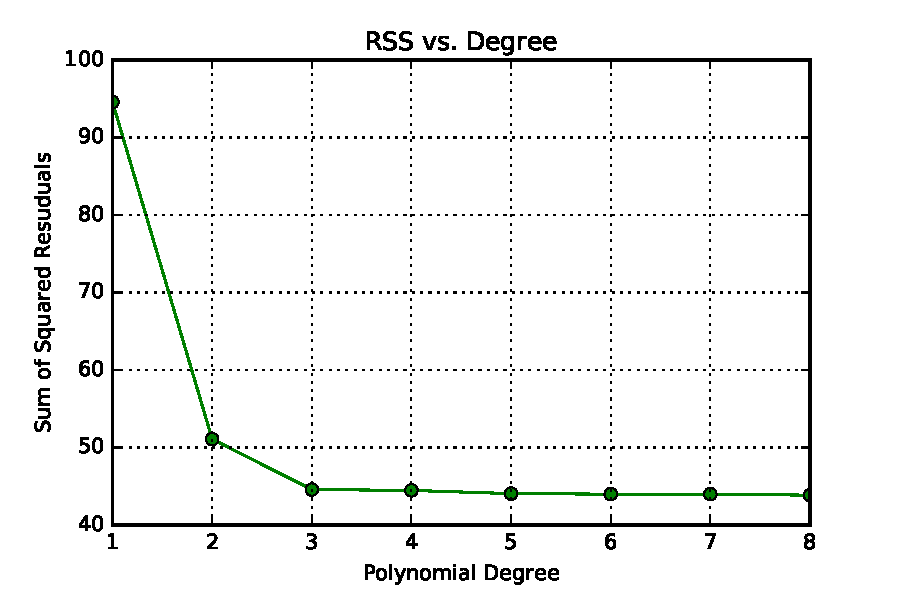
\includegraphics[width=0.9\textwidth]{./figures/rss.pdf}
\caption{\label{fig:RSS} RSS for different models}
\end{figure}
 
As shown in Figure \ref{fig:RSS}, the "elbow" point is at the degree 3. After 3, the RSS almost keep the same. In the following part, we plot the fitted curve for degree from 1 to 3.

For regression with degree 1, the result is shown in Figure \ref{fig:poly_1}. The corresponding RSS is 95.0 and the exact model is:
$$y = 5.6796 + 0.09948 * x $$ 
 
For regression with degree 2, the result is shown in Figure \ref{fig:poly_2}. The corresponding RSS is 51.0 and the exact model is:
$$y = -1.52544 + 0.27914 * x - 0.001006 * x^2 $$

For regression with degree 2, the result is shown in Figure \ref{fig:poly_3}. The corresponding RSS is 45.0 and the exact model is:
$$y = -9.40578 + 0.589406 * x - 0.00467882 * x^2  + 1.34768 * x^3 $$

\begin{figure}[H]
\centering
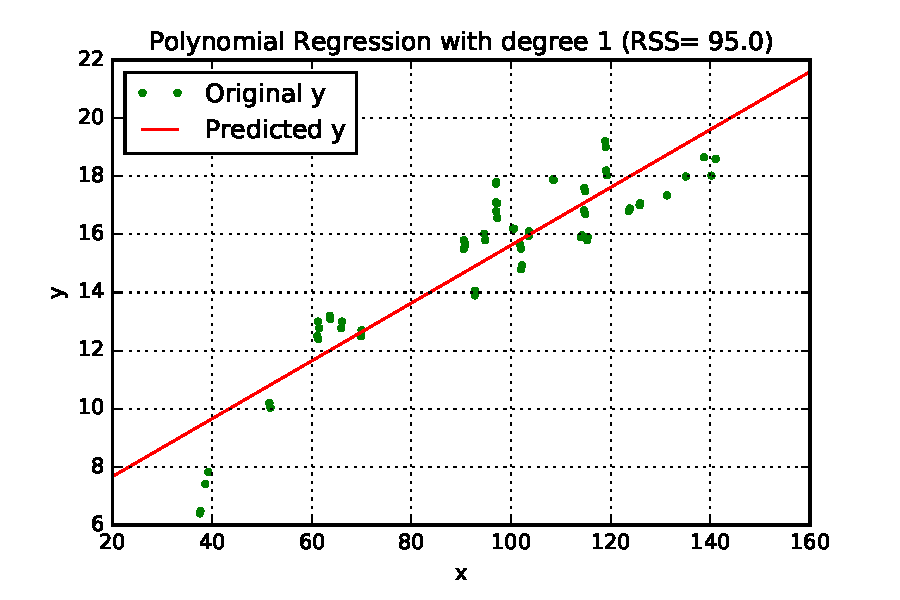
\includegraphics[width=0.9\textwidth]{./figures/poly_1.pdf}
\caption{\label{fig:poly_1} Polynomial regression with degree 1}
\end{figure}


\begin{figure}[H]
\centering
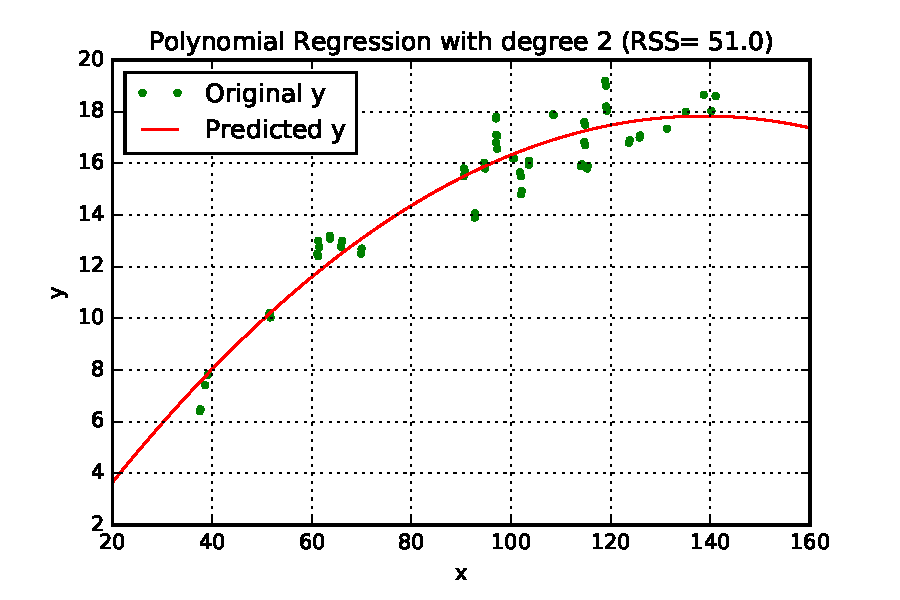
\includegraphics[width=0.9\textwidth]{./figures/poly_2.pdf}
\caption{\label{fig:poly_2} Polynomial regression with degree 2}
\end{figure}
 
 
\begin{figure}[H]
\centering
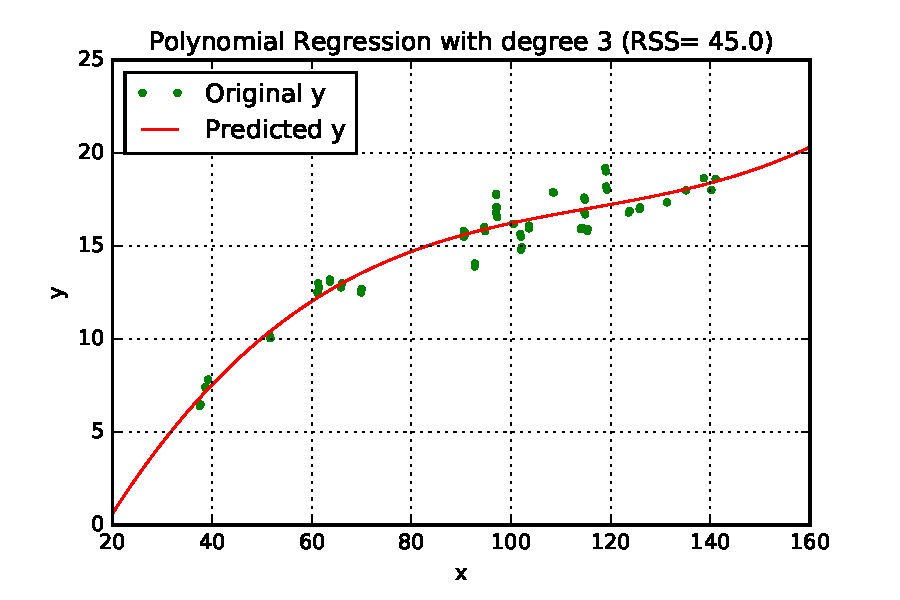
\includegraphics[width=0.9\textwidth]{./figures/poly_3.pdf}
\caption{\label{fig:poly_3} Polynomial regression with degree 3}
\end{figure}
 
\end{description}


\section*{\Large \Romannum{2}. Principal Component Analysis}
\begin{description}
\item{1. }
In this section, we applied the PCA model on the given data.

Suppose the input data has n sample and m features, then the input data can be expressed as an matrix X with dimension n by m. 
$$X = \begin{bmatrix}
	x_{11} & x_{12} & \cdots & x_{1m} \\
	x_{21} & x_{22} & \cdots & x_{2m} \\
	\vdots & \vdots & \vdots & \vdots \\
	x_{n1} & x_{n2} & \cdots & x_{nm} \\
\end{bmatrix}
$$

First, we de-mean the input data through calculating the mean value for each column and subtracting the mean value from each column $\tilde{x_{ij}} = x_{ij} - \bar{x_j}$, this can guarantee that each column of X has zero-mean. (In addition, if standardizing is required, we should also calculate the standard derivation from each column and divide each column by corresponding standard deviation $\tilde{x_{ij}} = \frac{x_{ij} - \bar{x_j}}{s_j}$).

In this way, the covariance matrix can be expressed as:
$$cov = \frac{X^T X}{n - 1}$$

Then, through SVD, we can get:
$$U, S, V = SVC(cov)$$

where each column of U is the eigenvector and the diagonal value of S is the corresponding variance. The implemented Python code is shown below.

\begin{lstlisting}
def PCA(x, whiten=False):
    """ function for Principal Component Analysis 
        
        x: shoule have the form of sample by feature
        whiten: if whiten = True, will standardized the input data
    """
    n, m = x.shape
    
    # de-mean the data
    x = x - np.mean(x, axis=0)
    if whiten == True:
        std = np.std(x, axis=0)
        x = x / std
    
    # compute the covariance matrix
    cov = np.dot(x.T, x) / (n - 1)
    
    # SVD
    u, s, v = np.linalg.svd(cov)
    ratio = s / np.sum(s)
    
    # project x onto the computed components
    projection = np.dot(x, u)
    
    return u, s, ratio, projection
\end{lstlisting}

\item{2. }
After calculating the eigenvector and the corresponding variance, for the non-standardized version, we can calculate the portion of each variance.
First, the 4 eigenvectors is:
$$
\begin{bmatrix}
 -0.36158968 & -0.65653988 &  0.58099728 &  0.31725455 \\
  0.08226889 & -0.72971237 & -0.59641809 & -0.32409435 \\
 -0.85657211 &  0.17576740 & -0.07252408 & -0.47971899 \\
 -0.35884393 &  0.07470647 & -0.54906091 &  0.75112056
\end{bmatrix}
$$ 

where each column is one eigenvector, the corresponding variance is:
$$\begin{bmatrix}
4.22484077 & 0.24224357 & 0.07852391 & 0.02368303
\end{bmatrix}$$

and the corresponding variance ration is :
$$\begin{bmatrix}
0.92461621 & 0.05301557 & 0.01718514 & 0.00518309
\end{bmatrix}$$

From above result, we can see that, the first two principal components can explain about 97.76\% of the total information, so keeping only the two components would be enough. In Figure \ref{fig:pca_1}

\begin{figure}[H]
\centering
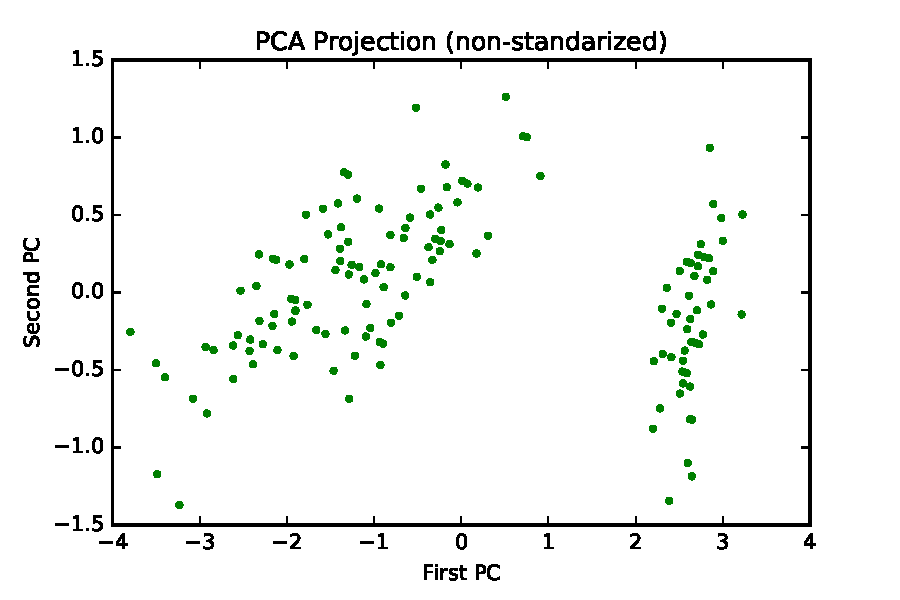
\includegraphics[width=0.9\textwidth]{./figures/projection1.pdf}
\caption{\label{fig:pca_1} PCA projection for non-standardized data}
\end{figure}

From above figure, we can notice that there are two visually apparent clusters and an intuitively guess is that there are two species. However, as we all know, for the Iris data, there actually has 3 species.\\

\item{2. }
For the standardized version, we can calculate the portion of each variance following the similar procedure, and the 4 eigenvectors is:
$$
\begin{bmatrix}
 -0.52237162 & -0.37231836 &  0.72101681 &  0.26199559 \\
  0.26335492 & -0.92555649 & -0.24203288 & -0.12413481 \\
 -0.58125401 & -0.02109478 & -0.14089226 & -0.80115427 \\
 -0.56561105 & -0.06541577 & -0.6338014  &  0.52354627
\end{bmatrix}
$$ 

where each column is one eigenvector, the corresponding variance is:
$$\begin{bmatrix}
2.93035378 & 0.92740362 & 0.14834223 & 0.02074601
\end{bmatrix}$$

and the corresponding variance ration is :
$$\begin{bmatrix}
0.72770452 & 0.23030523 & 0.03683832 & 0.00515193
\end{bmatrix}$$

From above result, we can see that, the first two principal components can explain about 95.80\% of the total information, so keeping only the two components would be enough. In Figure \ref{fig:pca_2}. The exact value is a little different from the result from the non-standardized version, but the projection is pretty similar to the previous result.

\begin{figure}[H]
\centering
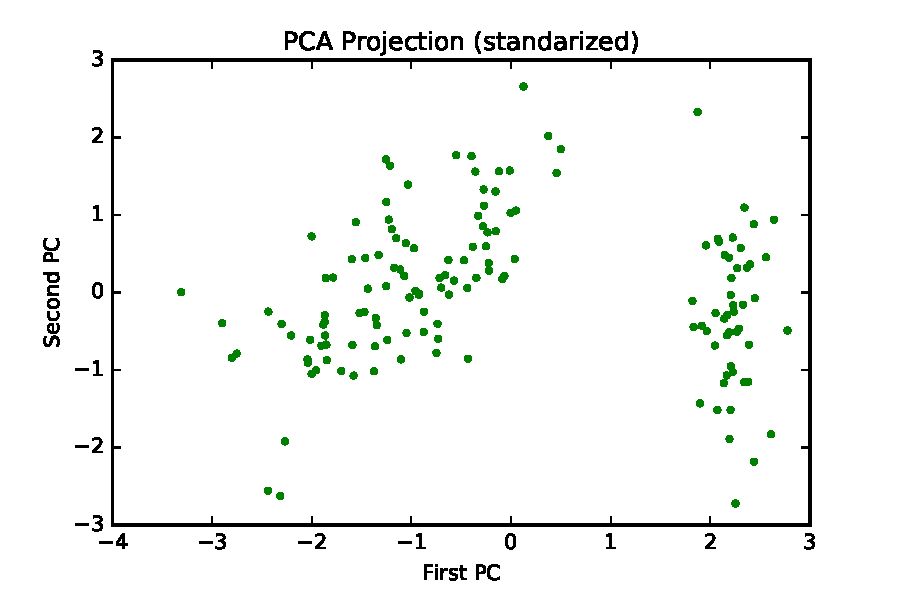
\includegraphics[width=0.9\textwidth]{./figures/projection2.pdf}
\caption{\label{fig:pca_2} PCA projection for standardized data}
\end{figure}

\end{description}

From above figure, we can notice that there are still two visually apparent clusters and an intuitively guess is that there are two species.


\newpage
%\begin{figure}[H]
%\centering
%\includegraphics[width=1.0\textwidth]{./images/detector}
%\caption{\label{fig:detector_system} Single detector system}
%\end{figure}


\clearpage

%\bibliographystyle{plain}
%\bibliographystyle{unsrt}
%\bibliography{reference.bib}

\end{document}

